\documentclass[11pt]{article}
\usepackage[utf8]{inputenc}


\usepackage{url}
\usepackage{breakurl}
\usepackage[breaklinks]{hyperref}
\usepackage[super]{nth}
\usepackage{bm}
\usepackage{booktabs}
\usepackage{enumerate}
\usepackage{graphicx}
\usepackage{multirow}
\usepackage{multicol}
\usepackage{amsmath}
\usepackage{amstext}
\usepackage{amssymb}
\usepackage{pdflscape}
\usepackage{multirow}
\usepackage{amsfonts}
\usepackage{rotating}
\usepackage{xcolor}
\usepackage{placeins}
\usepackage{amssymb}
\usepackage{listings}
\usepackage{xcolor}

\definecolor{codegreen}{rgb}{0,0.6,0}
\definecolor{codegray}{rgb}{0.5,0.5,0.5}
\definecolor{codepurple}{rgb}{0.58,0,0.82}
\definecolor{backcolour}{rgb}{0.95,0.95,0.92}

\lstdefinestyle{mystyle}{
    backgroundcolor=\color{backcolour},   
    commentstyle=\color{codegreen},
    keywordstyle=\color{magenta},
    numberstyle=\tiny\color{codegray},
    stringstyle=\color{codepurple},
    basicstyle=\ttfamily\footnotesize,
    breakatwhitespace=false,         
    breaklines=true,                 
    captionpos=b,                    
    keepspaces=true,                 
    numbers=left,                    
    numbersep=5pt,                  
    showspaces=false,                
    showstringspaces=false,
    showtabs=false,                  
    tabsize=2
}

\lstset{style=mystyle}
%\usepackage{algpseudocode}
\usepackage{natbib}
\usepackage{setspace} 
\usepackage{latexsym}
\usepackage{subfig}
\allowdisplaybreaks
\usepackage{array}
%\usepackage{subcaption}
\newcolumntype{H}{>{\setbox0=\hbox\bgroup}c<{\egroup}@{}}
\usepackage{pdfpages}
\usepackage{diagbox}
\usepackage{graphicx}
\usepackage{soul}

\usepackage{capt-of}% or \usepackage{caption}
\usepackage{varwidth}
\newsavebox\tmpbox

\usepackage{csvsimple,booktabs}
\usepackage{filecontents}

\usepackage{afterpage}
\graphicspath{{Images/}}


\usepackage{geometry}
\geometry{
	a4paper,
	total={160mm,220mm},
	left=16mm,
	top=22mm,
	bottom=30mm,
}

\usepackage[linesnumbered,ruled,vlined]{algorithm2e, algorithmic}

% Keywords command
\providecommand{\keywords}[1]
{
  \small	
  \textbf{\textit{Keywords---}} #1
}

\title{Campaign Optimization in Telecommunication Networks\\}
\author{Dursun Koc $^{a}$ \\ 
	dursun.koc@turkcell.com.tr, \\\\
	Dilek Gunnec $^{a}$ $^{\ast}$\\ 
	dilek.gunnec@ozyegin.edu.tr, ORCID ID: 0000-0002-0749-2584 \\\\
$^{a}$ Ozyegin University, Department of Industrial Engineering, Istanbul, Turkey \\ 
$^{\ast}$ Corresponding author \\ }
	
\date{}

\begin{document}
\maketitle
\begin{abstract}
For marketers, the main objective is to introduce their companies products or services to their customers or potential customers. Most of the studies, prior to this study, were on how to find the right audience for a marketing campaign. However, after finding the right target audience for a campaign, planing the communication to the target audience is also an important task. Such a plan should be fine-tuned not to irritate customers by sending too many messages, considering the communication channels' capacities, and it should also be compliant with the governments' regulations on marketing activities as well. In this study we propose a mathematical model which considers various communication limitations, and communication channels' capacities. In order to solve such a problem we propose a basic greedy heuristic, and a linear programming relaxation heuristic; later, we improved the greedy heuristic by implementing a small-scale linear programming model for finding a rough estimation for the expected number of communication for each campaign.\end{abstract}\hspace{10pt}

\keywords{Campaign Optimization, Telecommunication Networks, Greedy Heuristic.}

\newpage

\section{Introduction}

Companies conduct marketing activities to inform people about their products and services. Such activities are mostly done through marketing campaigns, and marketing campaigns are considered to be in the key role for increasing the market share or even gaining the market dominance \citep{xiao}. With the advancements in technology, marketers find great possibilities to reach their customers. Starting from the beginning of the 2000s digital marketing which can be defined as marketing on digital platforms, has converted conventional marketing into interactive, metric-based, objective, and relational way \citep{krishen}. It use various channels such as social media, SMS, e-mail, mobile apps(push-notification), search engines to touch the customers. Moreover in today's world with the aim of attracting the customer, marketers use all possibilities of technology with the inclusion of data science, artificial intelligence and internet of things \citep{buhalis}. However excessive and uncontrolled use of those channels may result in some drawbacks both in terms of regulations, and customer experience. Even sometimes misuse of customer data may cause irrelevant or irritating offers to customer \citep{malthouse}. So, each campaign has limitations and a specific target audience to reach. These limitations and restrictions prevent arbitrary and direct access to each individual in the target audience.\\

Performance of a campaign can be measured in two dimensions. The First dimension is the content of the campaign, setup for the campaign should be creative and attractive for customers. The Second dimension is the coverage in the target audience. However the attractiveness or the coolness of a campaign has limited effect on the success\citep{altshuler}, most of the time the success of a campaign can be defined as reaching the maximum portion of the target audience without breaking any limitations. \\

Most of the time the marketer does not need to send a direct message to the target audience in order to make them know about the campaign. If the marketer sends a message to a specific person who might talk about the campaign to some others, then the marker indirectly make those some others be aware about. A customers experience can be a reference for some others' opinion on a brands image. We know people share their knowledge, and ideas they have with others to whom they are connected socially, so we should consider these relations more than a conversation between two ordinary persons, such activities are enclosed in networks of relationships \citep{webster}. From the early days of network science it is considered to be an important tool for marketing \citep{arabie, webster}. \\

In this study we focus on solving a campaign optimization problem which we studied earlier. The campaign optimization problem is to maximize the effect of campaign in the target audience by touching directly or indirectly each customers, without violating any communication limitations have been put by customer experience experts and the legal regulations.\\

The remaining of this paper is structured as follows. In \S \ref{s:literature-review}, we review the related literature. In \S \ref{s:problem-model}, we describe the problem in detail and present our mathematical model for the problem. In \S \ref{s:solution-method}, we explain our proposed solution methods. In \S \ref{s:net-effect}, we introduce network effects to the problem. In \S \ref{s:num-analysis}, we present our computational results. Finally, we conclude in \S \ref{s:conclusion}.

%%%%%%%%%%%%%%%%%%%%%%%%%%%%%%%%%%%%%%%%%%%%%%%%%%%%%%%%%%
%%%%%%%%%%%%%%%%%%%%%%%%%%%%%%%%%%%%%%%%%%%%%%%%%%%%%%%%%%

\section{Literature Review}  \label{s:literature-review}

Although studies related to campaign management are common in marketing, there is increasing interest to this area from operations research and computer science areas, as the abundant data require complex data analysis skills. In my thesis, after such data analysis, we plan to introduce optimization methods which are not yet commonly used to tackle such problems. Specifically, one of our main contributions will be utilizing from network optimization tools to produce high quality solutions.\\

In this study, we plan to develop a model which tries to maximize the number of interactions for the campaigns decided by marketing team, while not exceeding the communication limitations. In the second place, we also try to increase the number of interaction to the most influential customers. We believe that influential customers can spread our message to a broader audience. In order to find the influential customer we will use customers' call and product purchase data from Turkcell.

\section{Problem Definition and Mathematical Model}  \label{s:problem-model}

In this section, we describe the proposed mathematical model to maximize the number of interactions to customers by adhering the communication limitations. In \S \ref{s:problem-desc}, we detail the limitations to customer communication and in \S \ref{s:problem-math}, we present our mathematical model.

\subsection{Problem Description} \label{s:problem-desc}

Turkcell, a telecommunication company in Turkey, provides different tariffs, services and products to its customers. In order to introduce these services and products to its existing and potential customers, the marketing team launches daily and weekly campaigns. A campaign can be seen as a marketing activity to introduce a product or a service to a predefined customer group through a set of communication channels within a specific period of time. Most of the time the product or the service can be offered with some advantages, like free usage or price advantages. But despite these benefits, customers may find campaign messages annoying. Before launching these campaigns, they analyze customer data to find the right target group. Then, they apply a set of business rules to optimize their communication with them. During this optimization process, several filters are used to keep the communication in certain frequency so that the customers are not disturbed frequently and with information unrelated to their needs. The first filter assures that no customers is informed about the same campaign from different channels. The second, limits the number of total interactions to a customer in one day. Campaigns are categorized in two dimensions; the first dimension is quota categories which describes filters for a campaign and the second one is priority categories which describes the importance of a campaign. Each campaign belongs to a quota category and each quota category has a limitation on the number of messages sent to a customer, both in a daily, and a weekly basis; moreover each campaign has a limitation unique to its own; and finally, each communication channel has a capacity that should not be exceeded for each day. Each campaign is bound to a priority category.\\

Turkcell launches about 70 campaigns on average for around 60-70 million customers through 3 channels each day, and these campaigns are planned in a weekly basis. Number of quota categories is fixed to 3, but priority categories can be variable around 10.\\

We study Turkcell’s outbound campaign management, and use an initial model to maximize the number of campaigns while abiding the rules for reaching to customers.

\subsection{Mathematical Model} \label{s:problem-math}

In this section, we present an integer programming model for the campaign optimization problem described at \S \ref{s:problem-desc}. We first introduce the notation and then present the model.\\

% General Math Model
\noindent \textbf{Sets}\\

\noindent ${\mathcal{C}}$: Set of campaigns \\
\noindent ${\mathcal{U}}$: Set of customers \\
\noindent ${\mathcal{H}}$: Set of channels \\
\noindent ${\mathcal{D}}$: Set of planning days \\
\noindent ${\mathcal{I}}$: Set of quota categories \\
\noindent ${\mathcal{P}}$: Set of priority categories \\


\noindent \textbf{Decision Variables}\\

\noindent $X_{{c}{u}{h}{d}}=1$, if message on campaign $c \in \mathcal{C}$ will be sent to customer $u \in \mathcal{U}$ through channel $h \in \mathcal{H}$ on day $d \in \mathcal{D}$, and 0 otherwise.\\

\noindent \textbf{Parameters}\\

\noindent $e_{{c}{u}}=1$, if customer $u \in \mathcal{U}$ is eligible for campaign $c \in \mathcal{C}$, and 0 otherwise.\\

\noindent $s_{{c}{u}{h}{d}}=1$, if customer $u \in \mathcal{U}$ is reached about campaign $c \in \mathcal{C}$, through channel $h \in \mathcal{H}$, on day $d \in \mathcal{D}$ the previous week and 0 otherwise.\\

\noindent $q_{{i}{c}}=1$, if campaign $c \in \mathcal{C}$ is in quota category $i \in \mathcal{I}$, and 0 otherwise.\\

\noindent $r_{{c}{p}}$ priority value of campaign $c \in \mathcal{C}$ regarding priority type $p \in \mathcal{P}$.\\

\noindent $b$ communication limit per customer for the planning horizon.\\

\noindent $k$ communication limit per customer for each day.\\

\noindent $l_{c}$ communication limit per customer for campaign $c \in \mathcal{C}$.\\

\noindent $m_{i}$ maximum number of times a customer can be contacted for quota category $i \in \mathcal{I}$ for the planning horizon.\\

\noindent $n_{i}$ maximum number of times a customer can be contacted for quota category $i \in \mathcal{I}$ on each day.\\

\noindent $t_{{h}{d}}$ capacity for channel $h \in \mathcal{H}$ on day $d \in \mathcal{D}$.\\

\noindent The formulation for the campaign optimization is presented next.

\begin{align}
\text{IP: }\text{Maximize} & \displaystyle
\sum\limits_{p\in \mathcal{P}}
\sum\limits_{c\in \mathcal{C}}
\sum\limits_{u\in \mathcal{U}}
\sum\limits_{h\in \mathcal{H}}
\sum\limits_{d\in \mathcal{D}}
X_{{c}{u}{h}{d}}  r_{{c}{p}} \label{mathmodel_obj}&
\\
\text{subject to} \notag\\
&X_{{c}{u}{h}{d}} \leq e_{{c}{u}}&\forall c \in \mathcal{C}, \forall u \in \mathcal{U}, \forall h \in \mathcal{H}, \forall d \in \mathcal{D}, \label{mathmodel_eligibility}&\\
&\sum\limits_{h\in\mathcal{H}}X_{{c}{u}{h}{d}} \leq 1 &\forall c \in \mathcal{C}, \forall u \in \mathcal{U}, \forall d \in \mathcal{D}, \label{mathmodel_singlechannel}&\\
&\sum\limits_{h\in\mathcal{H}}\sum\limits_{c\in\mathcal{C}}\sum\limits_{d\in\mathcal{D}}X_{{c}{u}{h}{d}} \leq b &\forall u \in \mathcal{U}, \label{mathmodel_percustomercommlimit}&\\
&\sum\limits_{h\in\mathcal{H}}\sum\limits_{c\in\mathcal{C}}\left(\sum_{d=1}^{w}X_{{c}{u}{h}{d}} + \sum_{d=w+1}^{7}s_{{c}{u}{h}{d}}\right) \leq b &\forall u \in \mathcal{U}, \forall w \in [1,6], \label{mathmodel_percustomercommlimit_rh}&\\
&\sum\limits_{h\in\mathcal{H}}\sum\limits_{c\in\mathcal{C}}X_{{c}{u}{h}{d}} \leq k &\forall u \in \mathcal{U}, \forall d \in \mathcal{D}, \label{mathmodel_percustomercommlimit_day}&\\
&\sum\limits_{d\in\mathcal{D}}\sum\limits_{h\in\mathcal{H}}X_{{c}{u}{h}{d}} \leq l_{c} &\forall c \in \mathcal{C}, \forall u \in \mathcal{U}, \label{mathmodel_percustomercamplimit}&\\
&\sum\limits_{h\in\mathcal{H}}\left( \sum_{d=1}^{w}X_{{c}{u}{h}{d}} + \sum_{d=w+1}^{7}s_{{c}{u}{h}{d}}\right) \leq l_{c} &\forall c \in \mathcal{C}, \forall u \in \mathcal{U}, \forall w \in [1,6], \label{mathmodel_percustomercamplimit_rh}&\\
&\sum\limits_{d\in\mathcal{D}}\sum\limits_{h\in\mathcal{H}}\sum\limits_{c\in\mathcal{C}}X_{{c}{u}{h}{d}}  q_{{i}{c}} \leq m_{i} &\forall u \in \mathcal{U}, \forall i \in \mathcal{I}, \label{mathmodel_weeklyquotalimit}&\\
&\sum\limits_{h\in\mathcal{H}}\sum\limits_{c\in\mathcal{C}}q_{{i}{c}}\left(\sum_{d=1}^{w}X_{{c}{u}{h}{d}} + \sum_{d=w+1}^{7}s_{{c}{u}{h}{d}}\right) \leq m_{i} &\forall u \in \mathcal{U}, \forall i \in \mathcal{I}, \forall w \in [1,6], \label{mathmodel_weeklyquotalimit_rh}&\\
&\sum\limits_{h\in\mathcal{H}}\sum\limits_{c\in\mathcal{C}}X_{{c}{u}{h}{d}}  q_{{i}{c}} \leq n_{i} &\forall u \in \mathcal{U}, \forall d \in \mathcal{D}, \forall i \in \mathcal{I}, \label{mathmodel_dailyquotalimit}&\\
&\sum\limits_{u\in\mathcal{U}}\sum\limits_{c\in\mathcal{C}}X_{{c}{u}{h}{d}} \leq t_{{h}{d}} &\forall d \in \mathcal{D}, \forall h \in \mathcal{H}, \label{mathmodel_channellimit}&\\
&X_{{c}{u}{h}{d}} \in \{0,1\}&\forall c \in \mathcal{C}, \forall u \in \mathcal{U}, \forall h \in \mathcal{H}, \forall d \in \mathcal{D}, \label{mathmodel_integrity}
\end{align}\\

The objective function \eqref{mathmodel_obj} maximizes the prioritized campaign communication. Constraints \eqref{mathmodel_eligibility} ensure that the communication will be placed only when the customer is eligible for that campaign. Constraints \eqref{mathmodel_singlechannel} say that a customer should not be targeted for the same campaign from different channels. Constraints \eqref{mathmodel_percustomercommlimit} define an upper-bound on the total number of communication to each customer for the whole period; and constraints \eqref{mathmodel_percustomercommlimit_rh} extend the upper-bound on the total number of communication to each customer regarding the rolling horizons. Constraints \eqref{mathmodel_percustomercommlimit_day} define an upper-bound for total number of communication to each customer for a single day. Constraints \eqref{mathmodel_percustomercamplimit} define an upper-bound for total number of communication to each customer per campaign for the whole period; and constraints \eqref{mathmodel_percustomercamplimit_rh} extend the upper-bound for total number of communication to each customer per campaign regarding the previous period. Campaigns are grouped by their marketing purpose, and for each of these groups we have combined limitations. Constraints \eqref{mathmodel_weeklyquotalimit} draw a limitation on the number of communications about campaigns that fell in specific groups. $q_{{i}{c}}$ equals to 1 if the campaign $c$ is in category  $i$. Likewise, constraints \eqref{mathmodel_weeklyquotalimit_rh} limits the number of communications for campaign quota categories regarding previous period. Constraints \eqref{mathmodel_dailyquotalimit} ensures that the number of communications for campaign quota categories for each day is not exceeded. Constraint \eqref{mathmodel_channellimit} ensures that each communication channels' capacity are not exceeded; and finally constraint \eqref{mathmodel_integrity} ensures that the variable $X_{{c}{u}{h}{d}}$ is either 0 or 1.\\

Due to its complexity, large instances of the campaign optimization problem may not be solved quickly by using exact methods. To support time to market objectives of marketing teams, we developed a heuristic approach that can attain high-quality solutions within a reasonable duration.

%%%%%%%%%%%%%%%%%%%%%%%%%%%%%%%%%%%%%%%%%%%%%%%%%%%%%%%%%%
%%%%%%%%%%%%%%%%%%%%%%%%%%%%%%%%%%%%%%%%%%%%%%%%%%%%%%%%%%

\section{Including the Network Effects and Solution Method} \label{s:net-effect}
In this section, we will take into account the network effect to reach a broader audience for our campaigns. As we stated earlier, the purpose of a marketer in running campaigns is to make her message reach a wide audience. Our current mathematical model maximizes the number of direct messages to customers regarding the campaign priority; however, we know that when we send a message to a certain customer, it may also be heard by other customers. We will assume that the network we will use, will give us an insight that some customers influence others to learn about our products and services. If customer \textit{i} receives a message; she may cause another customer \textit{j} to learn about that message. As a result, we touch two customers by sending only one message.

In our current model, we have some criteria which keep us from touching every eligible customer, so we are to drop some customers from the lists to ensure those criteria, using the network data we will try to drop the customers whose network effect is much lesser than others. In order to make it clear, let's consider we have customers 1, 2 and 3 are all eligible to campaign c, and we can send a message to only one customer; if we knew that 2 and 3 are connected in a network, we can retain either 2 or 3. Because if customer 1 is retained, only a single customer will be reached; however if either customers 2 or 3 is retained, two people will be reached because they will influence each other.

\subsection{Mathematical Model with Network Effects} \label{s:network-modif-model}
In order to include network effects, we revise out model as follows. We first introduce the new notation and then present the new mathematical model.
\\
% Network Modified Math Model

\noindent \textbf{Decision Variables}\\

\noindent $X_{{c}{u}{h}{d}}=1$, if campaign $c \in \mathcal{C}$ will be sent to customer $u \in \mathcal{U}$ through channel $h \in \mathcal{H}$ at day $d \in \mathcal{D}$, and 0 otherwise.
($\forall c \in \mathcal{C}$, $\forall u \in \mathcal{U}$, $\forall h \in \mathcal{H}$, $\forall d \in \mathcal{D}$ )\\

\noindent $Z_{{c}{u}}=1$, if campaign $c \in \mathcal{C}$ will be received by customer $u \in \mathcal{U}$ either directly from the marketer or indirectly through another customer, and 0 otherwise.
($\forall c \in \mathcal{C}$, $\forall u \in \mathcal{U}$, $\forall h \in \mathcal{H}$, $\forall d \in \mathcal{D}$ )\\

\noindent \textbf{Parameters}\\

\noindent $a_{{u}{v}}=1$, if customers \textit{u} and \textit{v} are adjacent, and 0 otherwise.
($\forall u, v \in \mathcal{U}$)\\


\noindent The formulation for the campaign optimization considering network effect is presented next.

\begin{align}
\text{Maximize} & \displaystyle
\sum\limits_{p\in \mathcal{P}}\sum\limits_{c\in \mathcal{C}}\sum\limits_{u\in \mathcal{U}}Z_{{c}{u}} r_{{c}{p}} \label{mathmodel_w/n_obj}&
\\
\text{subject to} \notag\\
&Z_{{c}{u}} \leq \sum\limits_{h\in \mathcal{H}}\sum\limits_{d\in \mathcal{D}}(X_{{c}{u}{h}{d}}+\sum\limits_{v\in\mathcal{U}}X_{{c}{v}{h}{d}}a_{{u}{v}}) &&&\forall c \in \mathcal{C}, \forall u \in \mathcal{U},\label{mathmodel_w/n_netcoverage}
\\
&\text{Constraints \eqref{mathmodel_eligibility} to \eqref{mathmodel_integrity} }\notag
\end{align}\\

\subsection{Building A Social Network Using Tariff-Change Data Network}\label{s:micro-world-networks}
Call data records (CDR) are commonly used to represent a social network of an individual. They could include both very close friends and also acquaintances who have not met in person, but talked over the phone. In our study, we need to represent closer relationships where one can inform their neighbour about a campaign-related message they received from a company. To reach such close contacts, we use tariff-change histories in addition to CDR data. In this way, we seek for people who have switch their tariff around the same time, and assume that they are close friends, who talk to each other about new mobile plans, etc. More specifically, we will build another network using both tariff-change data and SNA. In our new network nodes will be the customers and the edges will be placed when two customers are adjacent in the CDR network, and when their tariff-changes occurs in the same time (i.e., within 7 days). The tariff of a customer describes which products and services she uses, and the tariff-change data keeps the history of changes of tariff of a customer.

\begin{figure}[htp]
    \centering
    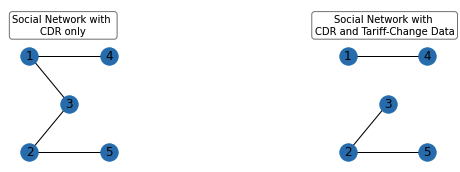
\includegraphics[height=5cm]{sample_sna_tsna.png}
    \caption{A Sample Social network modified with tariff-change data}
    \label{fig:fig_sample_sna}
\end{figure}
\begin{table}[htb]
    \centering
    \caption[Short Caption for LoT]{A Sample Tariff-Change History}\label{table:tbl_sample_tariff_change_history}
\csvautobooktabular{sample_tariff_change_history.csv}
\end{table}

Figure-\ref{fig:fig_sample_sna} shows a sample of social network constructed using CDR data, and Table-\ref{table:tbl_sample_tariff_change_history} gives a sample of tariff changes of customers in the SNA graph, in a time range of interest. From the tariff change history we can conclude that customer 1 and 4 should be connected; because customers 1 and 4 are changing tariff in the same period of time and they are connected in the SNA graph, likewise customers 2, 3 and 2, 5 are also connected because they are connected in the SNA graph and their tariff changes occurs in the same time periods. Even if customer 1 and 3 are connected in the SNA graph, they will not be connected in our final graph, because their tariff changes did not occur in the same time period.\\
 \\
\begin{algorithm}[H]
\DontPrintSemicolon
\KwIn{G:Social Network, DF: Tariff-Change Data, P: set of Products, T: Days threshold for co-occurrence. C: threshold for number of co-occurrences to build an edge}
\KwOut{G_{CDR}: Tariff-Change enriched Social Network}
\For{$u,v$ \gets $G$}{
    uvSalesCooccurance = 0\;
    \For{$p$ \gets $P$}{
        uSales = DF[u][p].dates\;
        vSales = DF[v][p].dates\;
        \If{$|uSales-vSales| \leq T$}{
           uvSalesCooccurance ++\;
        }
    }
    \If{$uvSalesCooccurance \geq C$}{
        $G_{CDR}.addEdge(u,v)$\;
    }
}
\Return{$G_{CDR}$}\;
\caption{Building Network using CDR and Tariff-Change Data}
\label{algo:building_net_cdr_tcd}
\end{algorithm}
\\ 
\\
We use algorithm-\ref{algo:building_net_cdr_tcd} in order to build a Social Network enriched with tariff-change data. We set a threshold of days difference value to identify two sales of tariff is related (\mathcal{T}), and also we set a threshold for number of co-occurrences of related tariff sales (\mathcal{C}) to add an edge between two customer. We start with an existing social network (\mathcal{G}) based on CDR data, a dataset of tariff-change history (\mathcal{DF}) which is bound to a set of products (\mathcal{P}).\\
We iterate through the connected (\mathcal{u,v}) pairs of \mathcal{G}. For every product \mathcal{p} we find the difference dates of sales for customers \mathcal{u}
, and \mathcal{v}, and if the difference exceeds the days threshold \mathcal{T} we increase the co-occurance counter (\mathcal{uvSalesCooccurance}) by 1. After covering the whole product set, we compare (\mathcal{uvSalesCooccurance}) with the threshold for number of co-occurances \mathcal{C}, and if (\mathcal{uvSalesCooccurance}) exceeds \mathcal{C}, we build an edge between customers \mathcal{u}, and \mathcal{v}.

\subsection{Solution Approach}
In this section first we modify our greedy heuristic algorithm at section-\ref{s:greedy_heuristic_improved} to solve the campaign optimization problem with network effect described at \S \ref{s:net-effect} and modelled at \S \ref{s:network-modif-model}. Later we will focus on how to sort customers in greedy approach, and we will try to solve some basic problems, and develop a heuristic algorithm. Finally at \S \ref{s:num-analysis} we will show computational study of the developed heuristic  result.

\subsubsection{Modified Greedy Algorithm}
The greedy algorithm described in \S \ref{s:greedy_heuristic_improved} assign customers in their index precedence; however when the network effect is to be considered we should assign the customers whose network precedence is greater, first.
\\
\begin{algorithm}[H]
\DontPrintSemicolon
\KwIn{X, $c\in\mathcal{C}$, $u\in\mathcal{U}$, $h\in\mathcal{H}$, $d\in\mathcal{D}$, $IPFeasibilityFunctions$ (constraints\eqref{mathmodel_eligibility} to \eqref{mathmodel_integrity})}
\KwOut{$X_{{c}{u}{h}{d}}$, $c\in\mathcal{C}$, $u\in\mathcal{U}$, $h\in\mathcal{H}$, $d\in\mathcal{D}$ such that constraints\eqref{mathmodel_eligibility} to \eqref{mathmodel_integrity} are satisfied}
  \SetKwFunction{FSortCampaigns}{SortCampaigns}
  \SetKwFunction{FCheckFeasibility}{CheckFeasibility}

  \SetKwProg{Fn}{Funtion}{:}{}
  \Fn{\FCheckFeasibility{$X$, $c$, $u$, $h$, $d$}}{
        FunctionsToCheck = $IPFeasibilityFunctions$ containig $X_{{c}{u}{h}{d}}$\;
        satisfied = FunctionsToCheck(X)\;
        \KwRet satisfied\;
  }\;
$Y_{{c}{d}}$ = Solve LP Model \eqref{mathmodel2_obj} to \eqref{mathmodel2_positive}

\For{$d \gets 1$ \textbf{to} $D$}{
SortCampaigns(C) \tcp*{such that($Y_{{c_{1}}{d}}  r_{c_{1}p} \geq Y_{{c_{2}}{d}}  r_{c_{2}p}$)}
    \For{$c \gets 1$ \textbf{to} $C$}{
        \For{$u \gets 1$ \textbf{to} \text{SortCustomersByNetworkPrecedence}($U$)}{
            \For{$h \gets 1$ \textbf{to} $H$}{
                 $X_{cuhd}$ = 1\;
                 \If {\textbf{not} CheckFeasibility(X,c,u,h,d)} {
                    $X_{cuhd}$ = 0\;
                 }
            }
        }
    }
}
\Return{$X$}\;
\caption{Greedy Heuristic improved by LP With Network Effect}
\label{algo:lprelax-net}
\end{algorithm}
\\
 At \S \ref{s:heu-camp-opt-with-net} we will focus on the implementation of \textit{SortCustomersByNetworkPrecedence} function at line 10 of algorithm-\ref{algo:lprelax-net}.\\
\subsubsection{Heuristics to Sort Customers By Network Precedence \label{s:heu-camp-opt-with-net}}

From the test instances at \S \ref{s:micro-world-networks}, we have concluded with the following algorithm-\ref{algo:cust-sort-a} which sorts nodes by their degree.

\begin{figure}[h!]
    \centering
    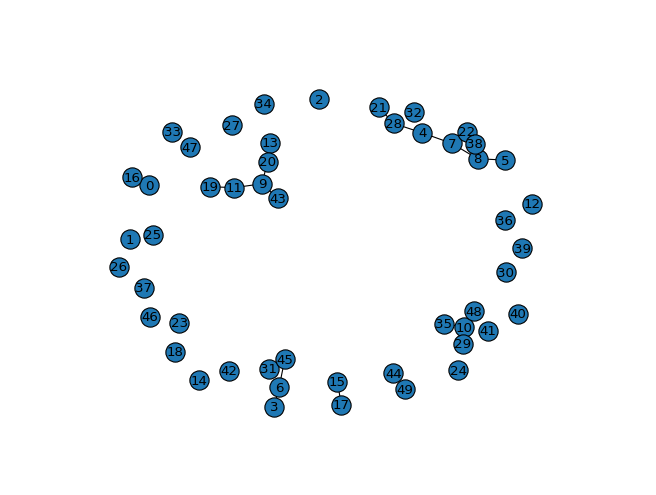
\includegraphics[width=12cm]{mini_world_case.png}
    \caption{Mini Network to Validate Heuristic}
    \label{fig:fig_mini_world_case}
\end{figure}

\begin{algorithm}[H]
\DontPrintSemicolon
\KwIn{G graph of customer network}
\KwOut{A Sorted list of customers $SC$}
$SC$ = []\;
\For{$u \in U$}{
  \State $N \gets ArgMax(G.degree)$\;
  \State $G.Remove(N)$\;
  \State $SC.Append(N)$\;
}
\Return {SC}\;
\caption{Customer Sorting-A for Greedy Approach for Campaign Optimization}
\label{algo:cust-sort-a}
\end{algorithm}
\\
\hbox{}
\\
In algorithm-\ref{algo:cust-sort-a} we sort customers by their degree centrality in the social network graph. In order to validate this algorithm we generated the following greater network than the ones at \S \ref{s:micro-world-networks}. A python implementation of algorithm-\ref{algo:cust-sort-a} can be seen at appendix-\ref{s:algo-impl-a}.\\

Open form of the mathematical model and optimal solution for the network is presented at appendix \ref{s:apendix-mini-net-cplex-sol}. Our criteria is to select at most 15 customers. The optimal solutions objective value is 348, however the objective value is 324 if we apply the algorithm-\ref{algo:cust-sort-a}, and selected customers were first fifteen of [7, 9, 10, 6, 28, 5, 11, 13, 15, 22, 31, 0, 1, 2, 3, 4, 8, 12, 14, 16, 17, 18, 19, 20, 21, 23, 24, 25, 26, 27, 29, 30, 32, 33, 34, 35, 36, 37, 38, 39, 40, 41, 42, 43, 44, 45, 46, 47, 48, 49]. \\

Our algorithm-\ref{algo:cust-sort-a}, selects a random customer when two customers degree centrality is equal, however selecting the one whose neighbours have not been selected would be much better. So we developed algorithm-\ref{algo:cust-sort-b} which pushes back a customer if that customers neighbour already selected. A python implementation of algorithm-\ref{algo:cust-sort-b} can be seen at appendix-\ref{s:algo-impl-b}.\\
\\
\\
\begin{algorithm}[H]
\KwIn{G graph of customer network}
\KwOut{A Sorted list of customers $SC$}
\State $SC \gets []$\;
\State $SS \gets []$\;

\For{$c \in C$}{
  \State $M \gets Max(G.degree)$\;
  \State $Ns \gets [G.degree == M]$\;
  \State $NNs \gets Ns.DropSeen(SS)$\;

  \If{$NNs.notEmpty$}{
    \State $SS.Append(G.neighbors(NNs[0]))$\;
    \State $SC.Append(NNs[0])$\;
    \State $G.Remove(NNs[0])$\;
  }
  \Else{
    \State $SS.Append(G.neighbors(Ns[0]))$\;
    \State $SC.Append(Ns[0])$\;
    \State $G.Remove(Ns[0])$\;
  }
  \EndIf
}
\Return {$SC$}
\caption{Customer Sorting-B for Greedy Approach for Campaign Optimization}
\label{algo:cust-sort-b}
\end{algorithm}
\\
\hbox{}
\\
Using algorithm-\ref{algo:cust-sort-b} we attained an objective value of 336, and selected customers were first fifteen of [7, 9, 10, 6, 28, 5, 13, 15, 19, 31, 38, 0, 1, 2, 12, 14, 16, 18, 23, 24, 25, 26, 27, 30, 32, 33, 34, 36, 37, 39, 40, 41, 42, 44, 46, 47, 49, 3, 4, 8, 11, 17, 20, 21, 22, 29, 35, 43, 45, 48].
\\
\hbox{}
\\
Finally we developed algorithm-\ref{algo:cust-sort-c} which uses a mathematical model whose aims is to find which customers should receive a direct message at least in order for a campaign message to reach all eligible customers.
\\
\hbox{}
\\
\noindent \textbf{Sets}\\

\noindent ${\mathcal{U}}$: set of customers. \\

\noindent \textbf{Decision Variables}\\

\noindent $W_{u}=1$, if customer $u \in \mathcal{U}$ should receive a direct, and 0 otherwise.
($\forall u \in \mathcal{U}$)\\

\noindent \textbf{Parameters}\\

\noindent $e_{u}=1$, if customer $u \in \mathcal{U}$ is eligible and 0 otherwise.
($\forall u \in \mathcal{U}$)\\

\noindent $a_{{u}{v}}=1$, if customer $u \in \mathcal{U}$ and customer $v \in \mathcal{U}$ and $u != v$, and 0 otherwise.
($\forall u \in \mathcal{U}$, $\forall v \in \mathcal{U}$, u != v)\\

\begin{align}
\text{Minimize} & \displaystyle
\sum\limits_{u\in \mathcal{U}}
W_{u} \label{mathmodel_net_cov_obj}&
\\
\text{subject to} \notag\\
&(W_{u}+\sum\limits_{v\in\mathcal{U}}W_{v}a_{{u}{v}}) \geq e_{u},&\forall u \in \mathcal{U} \label{mathmodel_net_cov_s1}
\\
&W_{u} \in \{0,1\},&\forall u \in \mathcal{U} \label{mathmodel_net_cov_integrity}
\end{align}\\

The objective function \eqref{mathmodel_net_cov_obj} minimizes the number of customers to receive the message. Constraints \eqref{mathmodel_net_cov_s1} ensure that each customers or its level-1 neighbour is touched, if it is eligible; and finally constraint \eqref{mathmodel_net_cov_integrity} ensure that the variable $W_{u}$ is either 0 or 1.\\

The preceding mathematical model is used for finding the minimum  customers to cover the whole network.

\begin{algorithm}[H]
\KwIn{G graph of customer network}
\KwIn{W customer list for min-vertex-cover}
\KwOut{A Sorted list of customers $SC$}
\State $SC \gets []$\;
\State $SS \gets []$\;

\For{$u \in U$}{
  \State $M \gets Max(G.degree-only-W)$\;
  \State $Ns \gets [G.degree \geq M]$\;
  \State $NNs \gets Ns.DropSeen(SS)$\;

  \If{$NNs.notEmpty$}{
    \State $SS.Append(G.neighbors(NNs[0]))$\;
    \State $SC.Append(NNs[0])$\;
    \State $G.Remove(NNs[0])$\;
  }
  \Else{
    \State $SS.Append(G.neighbors(Ns[0]))$\;
    \State $SC.Append(Ns[0])$\;
    \State $G.Remove(Ns[0])$\;
  }
  \EndIf
}
\EndFor
\Return {$SC$}
\caption{Customer Sorting-C for Greedy Approach for Campaign Optimization}
\label{algo:cust-sort-c}
\end{algorithm}

 A python implementation of algorithm-\ref{algo:cust-sort-c} can be seen at appendix-\ref{s:algo-impl-c}. Using algorithm-\ref{algo:cust-sort-c} we attained an objective value of 348 which is equal to the optimal solution, and selected customers were first fifteen of [10, 6, 8, 20, 22, 28, 15, 19, 43, 45, 0, 1, 2, 12, 14, 16, 18, 23, 24, 25, 26, 27, 30, 32, 33, 34, 36, 37, 39, 40, 41, 42, 44, 46, 47, 49, 3, 4, 5, 7, 9, 11, 13, 17, 21, 29, 31, 35, 38, 48].

\newpage
\section{Computational Study} \label{s:num-analysis}

In this section, we present the results of our computational study conducted to evaluate the performance of our greedy heuristic algorithms. We describe our test instances in \S \ref{test_cases}. We evaluate the performance of the greedy heuristics in \S \ref{test_evaluation}.

All computations were performed on a computer with 64-bit Windows 10 operating system with Intel(R) Core(TM) i7-3630QM CPU 16 GB RAM, and CPLEX 20.1 was used in Python to solve campaign optimization for exact results. Greedy heuristic algorithm is also coded in Python using Numpy library for fast mathematical operations.

%%%%%%%%%%%%%%%%%%%%%%%%%%%%%%%%%%%%%%%%%%%%%%%%%%%%%%%%%%
\subsection{Test Instances} \label{test_cases}
Table \ref{table:tbl_test_instances} shows the instances we tested our algorithms described at \S \ref{s:solution-method}. Instances from 1 to 4 can be regarded as low profile problems, instances from 5 to 9 can be seen as medium profile problems, instances from 10 to 14 can be seen as high profile problems, and instances 15 and 16 can be regarded as very high profile problem. A real world scenario can be 2 or 3 times bigger than the instance 16. In our test machine, problems greater than instance 14 cannot be executed using CPLEX solver.\\
 
\begin{table}[htb]
    \centering
    \caption[Short Caption for LoT]{Test instances for campaign optimization problem}\label{table:tbl_test_instances}
\csvautobooktabular{test_instances.csv}
\end{table}

\noindent \textbf{Parameters}\\

\noindent $e_{{c}{u}}$ is randomly generated $\mathcal{C} \times \mathcal{U}$ matrix having values 0 or 1,\\
\noindent $a_{{u}{v}}$ is randomly generated $\mathcal{U} \times \mathcal{U}$ matrix having values 0 or 1, representing a barabasi or erdos random network,\\
\noindent $q_{{i}{c}}$ is randomly generated $\mathcal{I} \times \mathcal{C}$ matrix having values 0 or 1,\\
\noindent $r_{{p}{c}}$ is randomly generated $\mathcal{P} \times \mathcal{C}$ matrix having values 0 to 100,\\
\noindent $b$ is set to 7,\\
\noindent $k$ is set to 3,\\
\noindent $l_c$ is randomly generated $\mathcal{C}$ length list having values 2, 3 or 4,\\
\noindent $m_i$ is randomly generated $\mathcal{I}$ length list having values 3, 4 or 5,\\
\noindent $n_i$ is randomly generated $\mathcal{I}$ length list having values 1, 2 or 3,\\
\noindent $t_{{h}{d}}$ is randomly generated $\mathcal{H} \times \mathcal{D}$ matrix having values $\mathcal{U}.5$, $\mathcal{U}.6$ or $\mathcal{U}.7$.\\

First, we executed instances from 1 to 14 using CPLEX MIP solver discarding the rolling horizon constraints (\ref{mathmodel_percustomercommlimit_rh}, \ref{mathmodel_percustomercamplimit_rh},  and \ref{mathmodel_weeklyquotalimit_rh}) and network effect described in \S \ref{s:net-effect} in the model in order to find the exact solution to the problem, later we solved the model including the rolling horizon constraints for instances from 1 to 11. Instances from 12 to 14 could not been solved with rolling horizon constraints; because for instances greater than 11 cannot be executed in our environment because of memory capacity.\\
Later we executed same instance using CLPEX LP solver in order to find the result for the lp-relaxation heuristic described at \S \ref{s:lp_relaxation_heuristic}.\\
In order to find the results for the basis greedy heuristic described at \S \ref{s:greedy_heuristic_basic} we executed instances from 1 to 16; and later for the same instances tested our improved greedy heuristic described at \S \ref{s:greedy_heuristic_improved} .
Finally we included the network effect to the problem using both barabasi and erdos random networks described at \S \ref{s:net-effect}, and run test instances from 1 to 10.

\subsubsection*{Preliminary Numerical Studies for Campaign Optimization with Network Effects}
We have conducted 6 different simulations, in each simulation the model contains only channel capacity constraint besides the network effect. Solutions provided by MIP Solver validates network effect, and it decided the customers whose degree centrality is greater than others, should receive the campaign messages. For each test instances we generate different random networks using either Erdos Renyi random network where each node is connected to another one with a probability of ${\mathcal{P}}$; or Barabasi Albert random network where each node is connected to ${\mathcal{M}}$ number of nodes. While using Barabasi Albert network we used a drop probability ${\mathcal{D}}$ to drop an edge to resemble that every connection may not carry a campaign message even if two customer are socially connected.\\
\begin{itemize}
\item Instance 1: Number of Customers: 10, Random Seed: 23, Network Type: barabasi, M:1, Edge Drop Propability: \%40.
\\
\begin{figure}[htp]
    \centering
    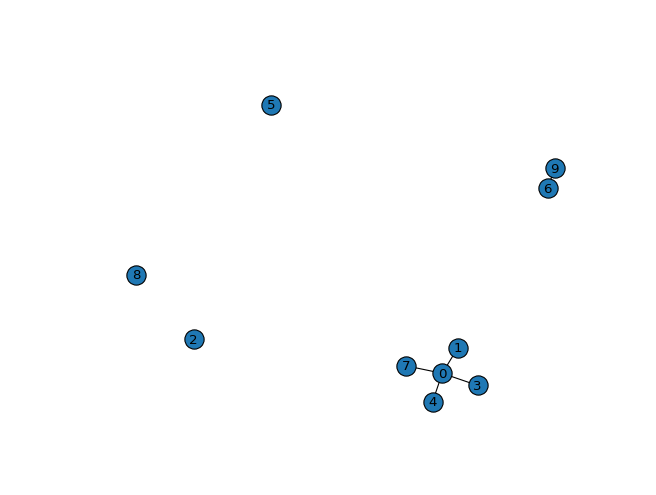
\includegraphics[width=6cm]{micro_world_case_1}
    \caption{Network for Instance 1}
    \label{fig:fig_micro_world_case_1}
\end{figure}
\\
MIP Solver solution offers customer-0 and customer-6 should receive the message.
We had 2 message capacity, and selected customer-0 whose degree-centrality measure is the greatest, later, we selected customer-6 which is connected customer-9. By sending 2 messages we can touch 7 customers.
\\
\item Instance 2: Number of Customers: 10, Random Seed: 45, Network Type: barabasi, M:1, Edge Drop Propability: \%10.
\\
\begin{figure}[htp]
    \centering
    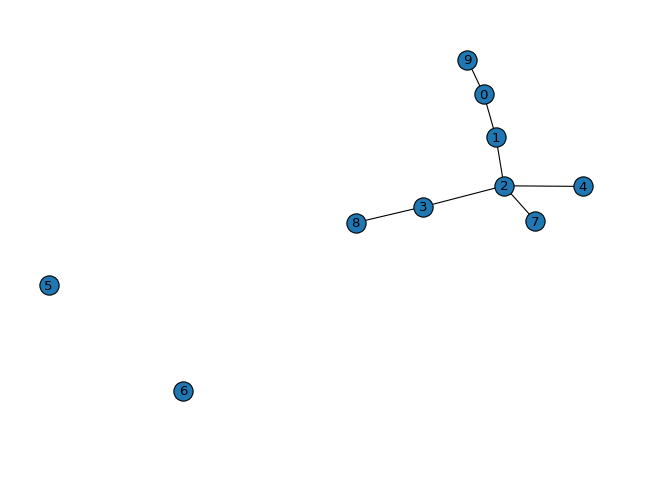
\includegraphics[width=6cm]{micro_world_case_2}
    \caption{Network for Instance 2}
    \label{fig:fig_micro_world_case_2}
\end{figure}
\\
MIP Solver solution offers customer-0 and customer-2 should receive the message.
We had 2 message capacity, and selected customer-2 whose degree-centrality measure is the greatest, later, we selected customer-0 which is connected customer-9 and customer-1. By sending 2 messages we can touch 7 customers.
\\
\item Instance 3: Number of Customers: 20, Random Seed: 83, Network Type: barabasi, M:2, Edge Drop Propability: \%80.
\\
\begin{figure}[htp]
    \centering
    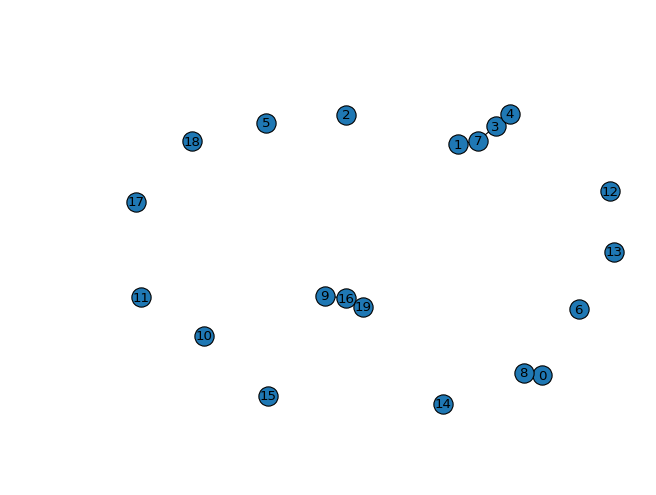
\includegraphics[width=6cm]{micro_world_case_3}
    \caption{Network for Instance 3}
    \label{fig:fig_micro_world_case_3}
\end{figure}
\\
MIP Solver solution offers customer-3 and customer-16 should receive the message.
We had 2 message capacity, and selected customer-16 whose degree-centrality measure is the one the greatest, later, we selected customer-3 which is connected customer-7 and customer-4. By sending 2 messages we can touch 6 customers.
\\
\item Instance 4: Number of Customers: 10, Random Seed: 42, Network Type: erdos, p:\%8.
\\
\begin{figure}[htp]
    \centering
    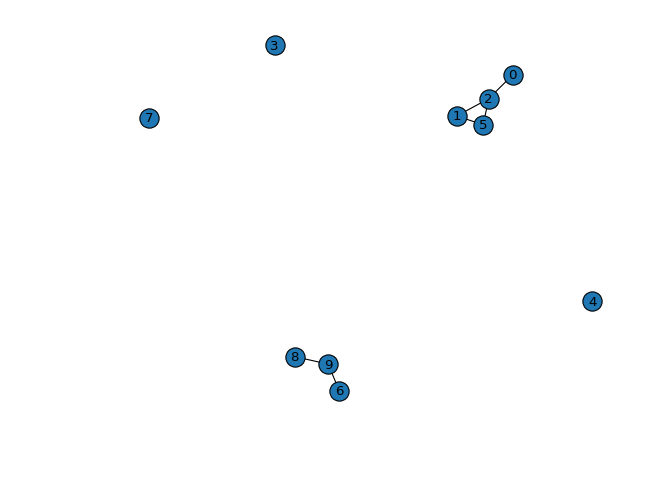
\includegraphics[width=6cm]{micro_world_case_4}
    \caption{Network for Instance 4}
    \label{fig:fig_micro_world_case_4}
\end{figure}
\\
MIP Solver solution offers customer-2, customer-3 and customer-9 should receive the message.
We had 3 message capacity, and selected customer-2 whose degree-centrality measure is the greatest, later, we selected customer-9 which is connected customer-8 and customer-6, and finally selected customer-3. By sending 3 messages we can touch 8 customers.
\\
\item Instance 5: Number of Customers: 10, Random Seed: 121, Network Type: erdos, p:\%4.
\\
\begin{figure}[htp]
    \centering
    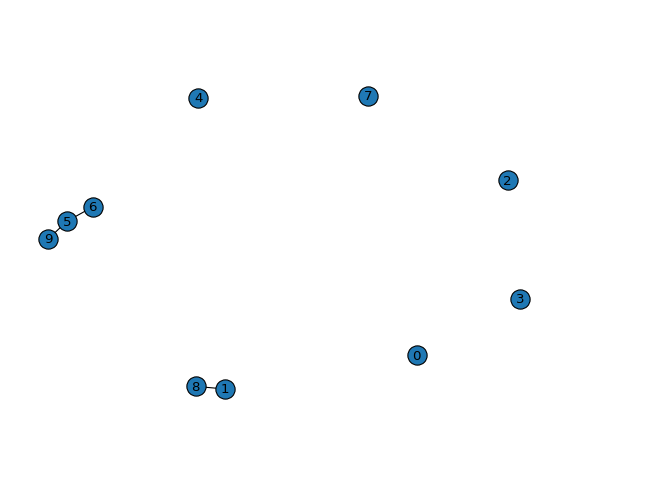
\includegraphics[width=6cm]{micro_world_case_5}
    \caption{Network for Instance 5}
    \label{fig:fig_micro_world_case_5}
\end{figure}
\\
MIP Solver solution offers customer-5 should receive the message.
We had 1 message capacity, and selected customer-5 whose degree-centrality measure is the greatest. By sending 1 messages we can touch 3 customers.
\\
\\

\item Instance 6: Number of Customers: 20, Random Seed: 142, Network Type: erdos, p: %3
Network.
\\
\begin{figure}[htp]
    \centering
    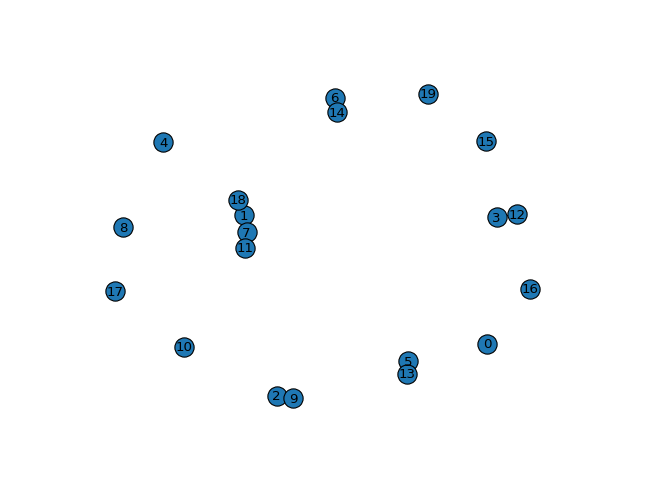
\includegraphics[width=6cm]{micro_world_case_6}
    \caption{Network for Instance 6}
    \label{fig:fig_micro_world_case_6}
\end{figure}
\\
MIP Solver solution offers customer-1, customer-2, customer-13 and customer-14 should receive the message.
We had 4 message capacity, and selected customer-1 whose degree-centrality measure is the greatest, later, we selected customer-2, customer-13 and customer-14 which are connected customers 9, 5 and 6 respectively. By sending 4 messages we can touch 9 customers.
\end{itemize}

\subsection{Results: Performance of the Greedy Heuristic and LP Relaxation Heuristic} \label{s:test_evaluation}
Table-\ref{table:tbl_test_durations_no_rh} and Figure-\ref{fig:fig_durations_no_rh} show duration in seconds for each method, and test instances, and Table-\ref{table:tbl_test_obj_diff_no_rh} and Figure-\ref{fig:fig_value_diff_no_rh} show  objective value of basic greedy, and LP-relaxation heuristics are differ from the exact solution's objective value. The differences are calculated using the formulation described at \S \ref{s:objective_value_assesment}.\\

For exact solution provided by CPLEX MIP solver the duration is exponentially increase as the problem size increases, and that increase become evident after instance-12. Objective value difference for LP-relaxation heuristic is almost invisible; however the objective value difference for basis greedy heuristic has more variations.\\

We executed test instance with rolling horizon constraints as well, Table-\ref{table:tbl_test_durations_with_rh_ph2} and Figure-\ref{fig:fig_durations_with_rh} show duration in seconds for each method and test instances, Table-\ref{table:tbl_test_obj_diff_with_rh_ph2} and Figure-\ref{fig:fig_value_diff_with_rh} shows the objective values of basis greedy, and LP-relaxation heuristics are differ from the exact solutions objective value respectively. Both performance figures and objective value differences are compatible with the ones with no rolling horizon values.\\

We executed test instances to test improved our greedy heuristic described at \S \ref{s:greedy_heuristic_improved}, Table-\ref{table:tbl_test_durations_bett_no_rh} and Figure-\ref{fig:fig_durations_bett_no_rh} show duration in seconds for each method and test instances, Table-\ref{table:tbl_test_obj_diff_bett_no_rh} and Figure-\ref{fig:fig_value_diff_bett_no_rh} shows the objective values of improved greedy, and LP-relaxation heuristics are differ from the exact solutions objective value respectively. Improved greedy heuristic seems to be worked as difference at instance-12 dropped from around \%16 to \%5, and instance-10 dropped from around \%4 to \%.2. We executed test instances 15 and 16 to see further performance of imporved greedy heuristic in durations, and it seems that the duration increased linearly.\\

In order to assess the solutions provided by heuristics against the exact solution, we calculate their distance to the exact solution using the formulation described at \equationautorefname \eqref{exact_distance_formulation}, and calculated objective value gaps are presented at table-\ref{table:tbl_test_obj_diff_no_rh}, table-\ref{table:tbl_test_obj_diff_with_rh_ph2}, and table-\ref{table:tbl_test_obj_diff_bett_no_rh}.\\

\noindent $V_{e}$: Exact objective value found by CPLEX-MIP solver. \\
\noindent $V_{h}$: Objective value found by heuristic. \\
\noindent $D_{h}$: Delta of heuristic result regarding exact solution. \\
\begin{align}
&D_{h} = 100 \frac{V_{e} - V_{h}}{V_{e}}, \label{exact_distance_formulation}&
\end{align}\\


During the execution of the model in CPLEX-MIP solution, and CPLEX-LP relaxation heuristics, the memory used increases more than 10GB with a cpu usage of around \%90, while the memory usage were limited to 300MB with a cpu usage around \%20 in both Basis Greedy heuristics, and the LP improved Greedy heuristics.\\

%%%%%%%%%%%%%%%%%%%%%%%%%%%%%%%%%%%%%%%%%%%%%%%%%%%%%%%%%%
%%%%%%%%%%%%%%%%%%%%%%%%%%%%%%%%%%%%%%%%%%%%%%%%%%%%%%%%%%

\afterpage{%
    \clearpage% Flush earlier floats (otherwise order might not be correct)
    \thispagestyle{empty}% empty page style (?)
    \begin{landscape}% Landscape page
        \begin{table}[htb]
                \centering
                \caption[Short Caption for LoT]{Execution time in secs - Discarding Rolling Horizon Constraints}\label{table:tbl_test_durations_no_rh}
            \csvautobooktabular{test_results_durations_no_rh.csv}
        \end{table}
        \begin{figure}[htp]
            \centering
            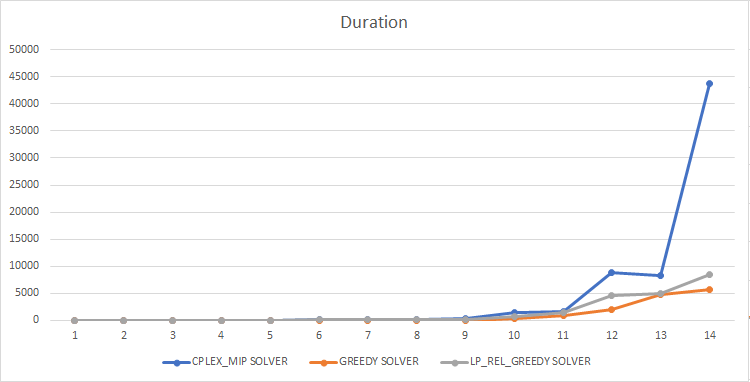
\includegraphics[width=12cm]{durations_no_rh}
            \caption{Execution time in secs - Discarding Rolling Horizon Constraints}
            \label{fig:fig_durations_no_rh}
        \end{figure}

        \begin{table}[htb]
                \centering
                \caption[Short Caption for LoT]{\% Objective Value Gap - Discarding Rolling Horizon Constraints}\label{table:tbl_test_obj_diff_no_rh}
            \csvautobooktabular{test_results_objective_diff_no_rh.csv}
        \end{table}
        \begin{figure}[htp]
            \centering
            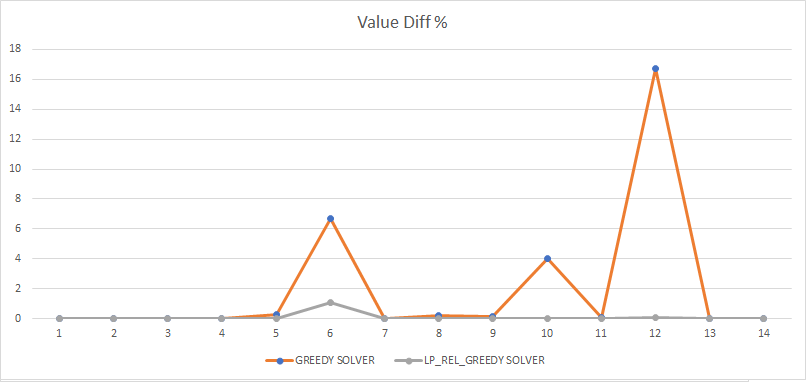
\includegraphics[width=12cm]{value_diff_no_rh}
            \caption{\% Objective Value Gap - Discarding Rolling Horizon Constraints}
            \label{fig:fig_value_diff_no_rh}
        \end{figure}
    \end{landscape}
\newpage
    \clearpage% Flush earlier floats (otherwise order might not be correct)
    \thispagestyle{empty}% empty page style (?)
    \begin{landscape}% Landscape page
        \begin{table}[htb]
                \centering
                \caption[Short Caption for LoT]{Execution time in secs - Considering Rolling Horizon Constraints}\label{table:tbl_test_durations_with_rh_ph2}
            \csvautobooktabular{test_results_durations_with_rh_ph2.csv}
        \end{table}
        
        \begin{figure}[htp]
            \centering
            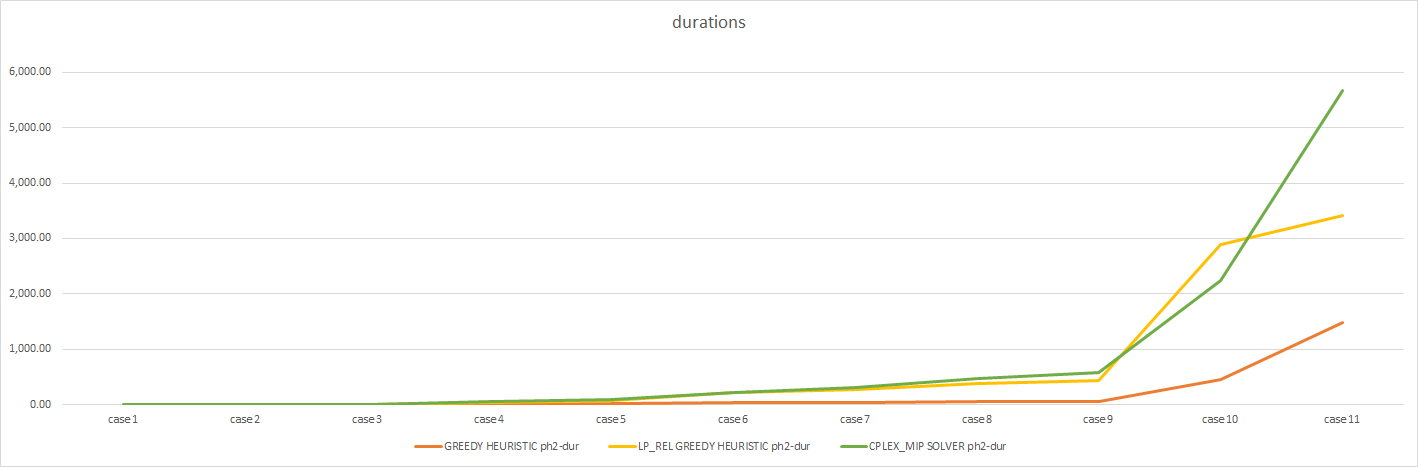
\includegraphics[width=20cm]{durations_with_rh}
            \caption{Execution time in secs - Considering Rolling Horizon Constraints}
            \label{fig:fig_durations_with_rh}
        \end{figure}
        
        \begin{table}[htb]
                \centering
                \caption[Short Caption for LoT]{\% Objective Value Gap - Considering Rolling Horizon Constraints}\label{table:tbl_test_obj_diff_with_rh_ph2}
            \csvautobooktabular{test_results_objective_diff_with_rh_ph2.csv}
        \end{table}
        \begin{figure}[htp]
            \centering
            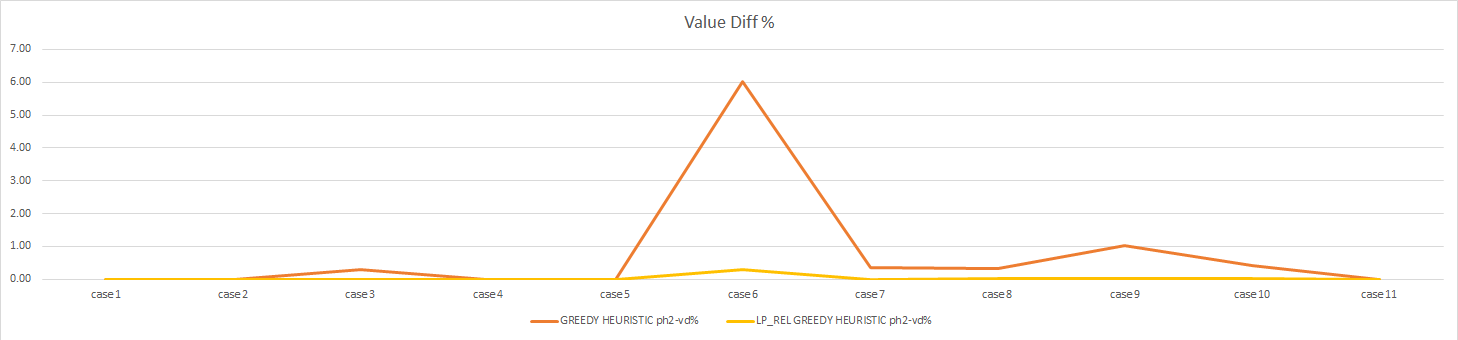
\includegraphics[width=20cm]{value_diff_with_rh}
            \caption{\% Objective Value Gap - Considering Rolling Horizon Constraints}
            \label{fig:fig_value_diff_with_rh}
        \end{figure}
    \end{landscape}
\newpage
    \clearpage% Flush earlier floats (otherwise order might not be correct)
    \thispagestyle{empty}% empty page style (?)
    \begin{landscape}% Landscape page
        \begin{table}[htb]
                \centering
                \caption[Short Caption for LoT]{Execution time in secs applying \ref{s:greedy_heuristic_improved} \textit{Greedy Heuristic improved by LP} - Discarding Rolling Horizon Constraints}\label{table:tbl_test_durations_bett_no_rh}
            \csvautobooktabular{test_results_durations_bett_no_rh.csv}
        \end{table}
        \begin{figure}[htp]
            \centering
            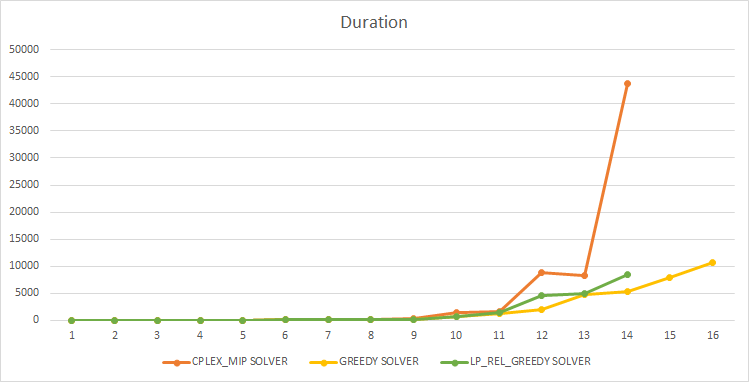
\includegraphics[width=12cm]{durations_bett_no_rh}
            \caption{Execution time in secs applying \ref{s:greedy_heuristic_improved} \textit{Greedy Heuristic improved by LP} - Discarding Rolling Horizon Constraints}
            \label{fig:fig_durations_bett_no_rh}
        \end{figure}

        \begin{table}[htb]
                \centering
                \caption[Short Caption for LoT]{\% Objective Gap applying \ref{s:greedy_heuristic_improved} \textit{Greedy Heuristic improved by LP} - Discarding Rolling Horizon Constraints}\label{table:tbl_test_obj_diff_bett_no_rh}
            \csvautobooktabular{test_results_objective_diff_bett_no_rh.csv}
        \end{table}
        \begin{figure}[htp]
            \centering
            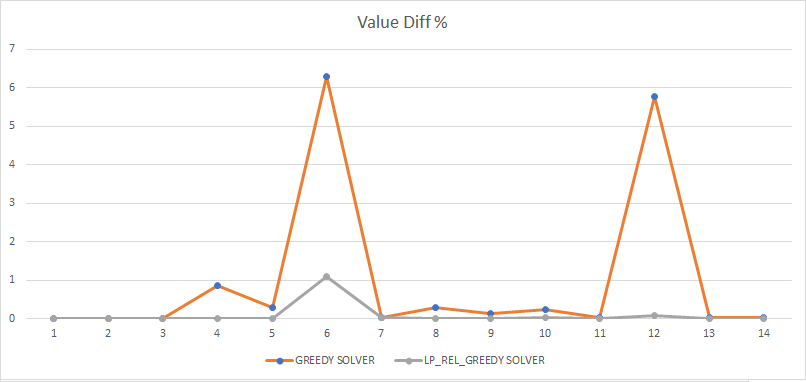
\includegraphics[width=12cm]{value_diff_bett_no_rh}
            \caption{\% Objective Gap applying \ref{s:greedy_heuristic_improved} \textit{Greedy Heuristic improved by LP} - Discarding Rolling Horizon Constraints}
            \label{fig:fig_value_diff_bett_no_rh}
        \end{figure}
    \end{landscape}
    \clearpage% Flush page
}

\newpage

\subsection{Results: Performance of the Greedy Heuristic When Network Effect Applied} \label{s:test_evaluation_net_effect}
We have generated random networks for following instances and present the solutions below. In basic Greedy approach we will be setting X values and using X values and ‘a’ value (adj. matrix) we will come up with Y values with the following formulation;

\begin{align}
X_{{c}{u}}=\sum\limits_{h\in \mathcal{H}}\sum\limits_{d\in \mathcal{D}}
X_{{c}{u}{h}{d}} \label{net_perf_conv_x} \\
Y_{{c}{u}}=[X_{{c}{u}} + \sum\limits_{v\in \mathcal{V}}
a_{{u}{v}}X_{{c}{u}}] > 0 \label{net_perf_conv_y}
\end{align}\\

In order to generate a erdos random network, we used random seed as 142, probability of edge creation as 0.03 and number of nodes as the number of customers for each instance, and in order to generate a barabasi random network, we used random seed as 142, attachement factor m as 3, drop probability as 0.9 and number of nodes as the number of customers for each instance.
Objective value gap when applying random network shown in table-\ref{table:tbl_test_obj_diff_with_net} and figure-\ref{fig:fig_value_diff_with_net} and number of edges per customer in both networks can be seen in table-\ref{table:tbl_edges_diff_erdos-barabsi}. We can infer that as number of connections per customer increases greedy algorithm seems to approximates to optimal solution much better. 

\begin{table}[htb]
        \centering
        \caption[Short Caption for LoT]{\% Objective Gap - Erdos Renyi vs Barabasi Random Network }\label{table:tbl_test_obj_diff_with_net}
    \csvautobooktabular{test_results_objective_diff_net_effect_erdos.csv}
\end{table}
\begin{figure}[htp]
    \centering
    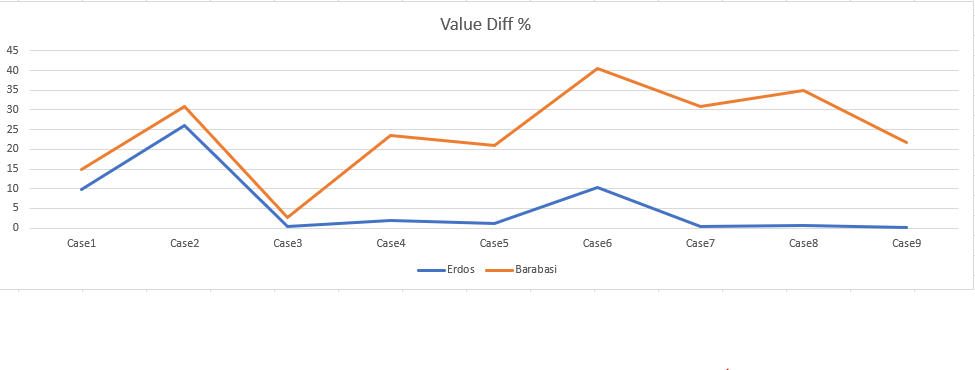
\includegraphics[width=12cm]{value_diff_with_net}
    \caption{\% Objective Gap  - Erdos Renyi vs Barabasi Random Network}
    \label{fig:fig_value_diff_with_net}
\end{figure}
\begin{table}[htb]
        \centering
        \caption[Short Caption for LoT]{\% Number of Edges per Customer - Erdos Renyi vs Barabasi Random Network }\label{table:tbl_edges_diff_erdos-barabsi}
    \csvautobooktabular{edges_diff_erdos-barabsi.csv}
\end{table}


%%%%%%%%%%%%%%%%%%%%%%%%%%%%%%%%%%%%%%%%%%%%%%%%%%%%%%%%%%
%%%%%%%%%%%%%%%%%%%%%%%%%%%%%%%%%%%%%%%%%%%%%%%%%%%%%%%%%%

\newpage

\section{Conclusion} \label{s:conclusion}
In this study, we discussed a campaign optimization problem, prior to this study literature mostly discussed the problems on finding right target audience, and optimization of it, against cost of delivery and return of investment. In this study our approach is to optimize an existing target audience against communication limitations, both not to irritate customer and be compliant with regulations such as GDPR. We mathematically modeled the problem described at \S \ref{s:problem-math} and later at \S \ref{s:solution-method} offered three heuristic to solve it. A greedy approach that starts with a small LP-model described at \S \ref{s:greedy_heuristic_improved} seems to find good solutions with-in reasonable duration with low memory and cpu.\\
Future research may focus on developing alternative solution methods for the proposed campaign optimization problem. In case of network effect current heuristic can be improved to decrease the gap to the optimal solution. Moreover, new methodologies can be offered to measure the effectiveness of the network.

\newpage

\appendix
\section{Appendices}
\subsection{Mathmetical Model and Solution for Mini Campaign Optimization Problem with Network Effect}\label{s:apendix-mini-net-cplex-sol}
========\\
Model:\\
========\\
Max:\\
        12Y[0,0]+12Y[0,1]+12Y[0,2]+12Y[0,3]+12Y[0,4]+12Y[0,5]+12Y[0,6]+12Y[0,7]+12Y[0,8]+12Y[0,9]+12Y[0,10]+12Y[0,11]+12Y[0,12]+12Y[0,13]+12Y[0,14]+12Y[0,15]+12Y[0,16]+12Y[0,17]+12Y[0,18]+12Y[0,19]+12Y[0,20]+12Y[0,21]+12Y[0,22]+12Y[0,23]+12Y[0,24]+12Y[0,25]+12Y[0,26]+12Y[0,27]+12Y[0,28]+12Y[0,29]+12Y[0,30]+12Y[0,31]+12Y[0,32]+12Y[0,33]+12Y[0,34]+12Y[0,35]+12Y[0,36]+12Y[0,37]+12Y[0,38]+12Y[0,39]+12Y[0,40]+12Y[0,41]+12Y[0,42]+12Y[0,43]+12Y[0,44]+12Y[0,45]+12Y[0,46]+12Y[0,47]+12Y[0,48]+12Y[0,49]\\
subject to:\\
        X[0,0,0,0] \leq 1.0\\
        X[0,1,0,0] \leq 1.0\\
        X[0,2,0,0] \leq 1.0\\
        X[0,3,0,0] \leq 1.0\\
        X[0,4,0,0] \leq 1.0\\
        X[0,5,0,0] \leq 1.0\\
        X[0,6,0,0] \leq 1.0\\
        X[0,7,0,0] \leq 1.0\\
        X[0,8,0,0] \leq 1.0\\
        X[0,9,0,0] \leq 1.0\\
        X[0,10,0,0] \leq 1.0\\
        X[0,11,0,0] \leq 1.0\\
        X[0,12,0,0] \leq 1.0\\
        X[0,13,0,0] \leq 1.0\\
        X[0,14,0,0] \leq 1.0\\
        X[0,15,0,0] \leq 1.0\\
        X[0,16,0,0] \leq 1.0\\
        X[0,17,0,0] \leq 1.0\\
        X[0,18,0,0] \leq 1.0\\
        X[0,19,0,0] \leq 1.0\\
        X[0,20,0,0] \leq 1.0\\
        X[0,21,0,0] \leq 1.0\\
        X[0,22,0,0] \leq 1.0\\
        X[0,23,0,0] \leq 1.0\\
        X[0,24,0,0] \leq 1.0\\
        X[0,25,0,0] \leq 1.0\\
        X[0,26,0,0] \leq 1.0\\
        X[0,27,0,0] \leq 1.0\\
        X[0,28,0,0] \leq 1.0\\
        X[0,29,0,0] \leq 1.0\\
        X[0,30,0,0] \leq 1.0\\
        X[0,31,0,0] \leq 1.0\\
        X[0,32,0,0] \leq 1.0\\
        X[0,33,0,0] \leq 1.0\\
        X[0,34,0,0] \leq 1.0\\
        X[0,35,0,0] \leq 1.0\\
        X[0,36,0,0] \leq 1.0\\
        X[0,37,0,0] \leq 1.0\\
        X[0,38,0,0] \leq 1.0\\
        X[0,39,0,0] \leq 1.0\\
        X[0,40,0,0] \leq 1.0\\
        X[0,41,0,0] \leq 1.0\\
        X[0,42,0,0] \leq 1.0\\
        X[0,43,0,0] \leq 1.0\\
        X[0,44,0,0] \leq 1.0\\
        X[0,45,0,0] \leq 1.0\\
        X[0,46,0,0] \leq 1.0\\
        X[0,47,0,0] \leq 1.0\\
        X[0,48,0,0] \leq 1.0\\
        X[0,49,0,0] \leq 1.0\\
        X[0,0,0,0]+X[0,1,0,0]+X[0,2,0,0]+X[0,3,0,0]+X[0,4,0,0]+X[0,5,0,0]+X[0,6,0,0]+X[0,7,0,0]+X[0,8,0,0]+X[0,9,0,0]+X[0,10,0,0]+X[0,11,0,0]+X[0,12,0,0]+X[0,13,0,0]+X[0,14,0,0]+X[0,15,0,0]+X[0,16,0,0]+X[0,17,0,0]+X[0,18,0,0]+X[0,19,0,0]+X[0,20,0,0]+X[0,21,0,0]+X[0,22,0,0]+X[0,23,0,0]+X[0,24,0,0]+X[0,25,0,0]+X[0,26,0,0]+X[0,27,0,0]+X[0,28,0,0]+X[0,29,0,0]+X[0,30,0,0]+X[0,31,0,0]+X[0,32,0,0]+X[0,33,0,0]+X[0,34,0,0]+X[0,35,0,0]+X[0,36,0,0]+X[0,37,0,0]+X[0,38,0,0]+X[0,39,0,0]+X[0,40,0,0]+X[0,41,0,0]+X[0,42,0,0]+X[0,43,0,0]+X[0,44,0,0]+X[0,45,0,0]+X[0,46,0,0]+X[0,47,0,0]+X[0,48,0,0]+X[0,49,0,0] \leq 15.0\\
        Y[0,0] \leq X[0,0,0,0]\\
        Y[0,1] \leq X[0,1,0,0]\\
        Y[0,2] \leq X[0,2,0,0]\\
        Y[0,3] \leq X[0,3,0,0]+X[0,6,0,0]\\
        Y[0,4] \leq X[0,4,0,0]+X[0,7,0,0]+X[0,28,0,0]\\
        Y[0,5] \leq X[0,5,0,0]+X[0,8,0,0]\\
        Y[0,6] \leq X[0,3,0,0]+X[0,6,0,0]+X[0,45,0,0]\\
        Y[0,7] \leq X[0,4,0,0]+X[0,7,0,0]+X[0,8,0,0]+X[0,22,0,0]\\
        Y[0,8] \leq X[0,5,0,0]+X[0,7,0,0]+X[0,8,0,0]\\
        Y[0,9] \leq X[0,9,0,0]+X[0,11,0,0]+X[0,20,0,0]+X[0,43,0,0]\\
        Y[0,10] \leq X[0,10,0,0]+X[0,29,0,0]+X[0,35,0,0]+X[0,48,0,0]\\
        Y[0,11] \leq X[0,9,0,0]+X[0,11,0,0]+X[0,19,0,0]\\
        Y[0,12] \leq X[0,12,0,0]\\
        Y[0,13] \leq X[0,13,0,0]+X[0,20,0,0]\\
        Y[0,14] \leq X[0,14,0,0]\\
        Y[0,15] \leq X[0,15,0,0]+X[0,17,0,0]\\
        Y[0,16] \leq X[0,16,0,0]\\
        Y[0,17] \leq X[0,15,0,0]+X[0,17,0,0]\\
        Y[0,18] \leq X[0,18,0,0]\\
        Y[0,19] \leq X[0,11,0,0]+X[0,19,0,0]\\
        Y[0,20] \leq X[0,9,0,0]+X[0,13,0,0]+X[0,20,0,0]\\
        Y[0,21] \leq X[0,21,0,0]+X[0,28,0,0]\\
        Y[0,22] \leq X[0,7,0,0]+X[0,22,0,0]+X[0,38,0,0]\\
        Y[0,23] \leq X[0,23,0,0]\\
        Y[0,24] \leq X[0,24,0,0]\\
        Y[0,25] \leq X[0,25,0,0]\\
        Y[0,26] \leq X[0,26,0,0]\\
        Y[0,27] \leq X[0,27,0,0]\\
        Y[0,28] \leq X[0,4,0,0]+X[0,21,0,0]+X[0,28,0,0]\\
        Y[0,29] \leq X[0,10,0,0]+X[0,29,0,0]\\
        Y[0,30] \leq X[0,30,0,0]\\
        Y[0,31] \leq X[0,31,0,0]+X[0,45,0,0]\\
        Y[0,32] \leq X[0,32,0,0]\\
        Y[0,33] \leq X[0,33,0,0]\\
        Y[0,34] \leq X[0,34,0,0]\\
        Y[0,35] \leq X[0,10,0,0]+X[0,35,0,0]\\
        Y[0,36] \leq X[0,36,0,0]\\
        Y[0,37] \leq X[0,37,0,0]\\
        Y[0,38] \leq X[0,22,0,0]+X[0,38,0,0]\\
        Y[0,39] \leq X[0,39,0,0]\\
        Y[0,40] \leq X[0,40,0,0]\\
        Y[0,41] \leq X[0,41,0,0]\\
        Y[0,42] \leq X[0,42,0,0]\\
        Y[0,43] \leq X[0,9,0,0]+X[0,43,0,0]\\
        Y[0,44] \leq X[0,44,0,0]\\
        Y[0,45] \leq X[0,6,0,0]+X[0,31,0,0]+X[0,45,0,0]\\
        Y[0,46] \leq X[0,46,0,0]\\
        Y[0,47] \leq X[0,47,0,0]\\
        Y[0,48] \leq X[0,10,0,0]+X[0,48,0,0]\\
        Y[0,49] \leq X[0,49,0,0]\\
========\\
Solution:\\
obj: 348.0\\
========\\
X[0,0,0,0] = 1.0\\
X[0,1,0,0] = 1.0\\
X[0,2,0,0] = 1.0\\
X[0,6,0,0] = 1.0\\
X[0,8,0,0] = 1.0\\
X[0,9,0,0] = 1.0\\
X[0,10,0,0] = 1.0\\
X[0,11,0,0] = 1.0\\
X[0,12,0,0] = 1.0\\
X[0,15,0,0] = 1.0\\
X[0,20,0,0] = 1.0\\
X[0,22,0,0] = 1.0\\
X[0,28,0,0] = 1.0\\
X[0,34,0,0] = 1.0\\
X[0,45,0,0] = 1.0\\
Y[0,0] = 1.0\\
Y[0,1] = 1.0\\
Y[0,2] = 1.0\\
Y[0,3] = 1.0\\
Y[0,4] = 1.0\\
Y[0,5] = 1.0\\
Y[0,6] = 1.0\\
Y[0,7] = 1.0\\
Y[0,8] = 1.0\\
Y[0,9] = 1.0\\
Y[0,10] = 1.0\\
Y[0,11] = 1.0\\
Y[0,12] = 1.0\\
Y[0,13] = 1.0\\
Y[0,15] = 1.0\\
Y[0,17] = 1.0\\
Y[0,19] = 1.0\\
Y[0,20] = 1.0\\
Y[0,21] = 1.0\\
Y[0,22] = 1.0\\
Y[0,28] = 1.0\\
Y[0,29] = 1.0\\
Y[0,31] = 1.0\\
Y[0,34] = 1.0\\
Y[0,35] = 1.0\\
Y[0,38] = 1.0\\
Y[0,43] = 1.0\\
Y[0,45] = 1.0\\
Y[0,48] = 1.0\\
========\\
\newpage

\subsection{Python implementation for Algorithm-\ref{algo:cust-sort-a} \label{s:algo-impl-a}}
\begin{lstlisting}[language=Python]
def max_degree(self, grph):
    nn = max(grph.degree, key=lambda x: x[1])
    grph.remove_node(nn[0])
    return nn[0]

def sort_nodes_to_inc_span(self, grph):
    return [self.max_degree(grph) for i in range(len(grph.nodes()))]
\end{lstlisting}

\subsection{Python implementation for Algorithm-\ref{algo:cust-sort-b} \label{s:algo-impl-b}}
\begin{lstlisting}[language=Python]
def max_degree_b(self, grph, seen):
    max_val = max(grph.degree, key=lambda x: x[1])[1]
    nns = [n for n in grph.degree if n[1] == max_val]
    nns_ = [n for n in nns if n[0] not in seen]
    if len(nns_)>0:
        nn = nns_[0]
    else:
        nn = nns[0]
    neighbors = grph.neighbors(nn[0])
    grph.remove_node(nn[0])
    seen |= set(list(neighbors))
    return (nn[0], seen)

def sort_nodes_to_inc_span(self, grph):
    result=list()
    seen = set()
    for _ in range(len(grph.degree)):
        elem, seen = self.max_degree_b(grph, seen)
        result.append(elem)
    return result
\end{lstlisting}

\subsection{Python implementation for Algorithm-\ref{algo:cust-sort-c} \label{s:algo-impl-c}}
\begin{lstlisting}[language=Python]
def max_degree_b(self, grph, seen, X_u):
    dd = {gd[0]:gd[1]*X_u[gd[0]] for gd in grph.degree}
    max_val = max(dd.items(), key=lambda x: x[1])[1]
    nns = [n for n in dd.items() if n[1] == max_val]
    nns_ = [n for n in nns if n[0] not in seen]
    if len(nns_)>0:
        nn = nns_[0]
    else:
        nn = nns[0]
    neighbors = grph.neighbors(nn[0])
    grph.remove_node(nn[0])
    seen |= set(list(neighbors))
    return (nn[0], seen)

def sort_nodes_to_inc_span(self, grph, X_u):
    result=list()
    seen = set()
    for _ in range(len(grph.degree)):
        elem, seen = self.max_degree_b(grph, seen, X_u)
        result.append(elem)
    return result
\end{lstlisting}


\newpage
\bibliographystyle{chicago}

\bibliography{references}

\end{document}